%文档类型
\documentclass[a4paper]{article}

%引用包裹
\usepackage{bm}
\usepackage{cmap}
\usepackage{ctex}
\usepackage{cite}
\usepackage{color}
\usepackage{float}
\usepackage{xeCJK}
\usepackage{amsthm}
\usepackage{amsmath}
\usepackage{amssymb}
\usepackage{setspace}
\usepackage{geometry}
\usepackage{hyperref}
\usepackage{enumerate}
\usepackage{indentfirst}
\usepackage[cache=false]{minted}
\usepackage{fontspec}
\usepackage{pdfpages}
\usepackage{fancyhdr}
%代码高亮
\geometry{margin=1in}
\setmonofont{Consolas}
%字体设置
\setmainfont{Consolas}
\setCJKmonofont{SimSun}
\setCJKmainfont[BoldFont={SimSun}]{SimSun}

\newcommand{\cppcode}[1]{
    \inputminted[mathescape,
    frame=lines,linenos]{cpp}{source/#1}
}

\newcommand{\javacode}[1]{
    \inputminted[mathescape,
    frame=lines,linenos]{java}{source/#1}
}
\title{代码库}
\author{Spear of Longinus}
\date{\today}

 
\begin{document}

\maketitle

\tableofcontents

\newpage

\section{数论}

\subsection{快速求逆元}

返回结果:$$x^{-1}(mod)$$
\indent 使用条件:$x \in [0, mod)$并且$x$与$mod$互质

\cppcode{number-theory/inverse.cpp}

\subsection{扩展欧几里德算法}


返回结果:$$ax+by=gcd(a,b)$$
\indent 时间复杂度:$\mathcal{O}(nlogn)$

\cppcode{number-theory/extended-euclid.cpp}

\subsection{中国剩余定理}

返回结果:$$x \equiv r_i (mod \ p_i) \ (0 \leq i < n)$$
\indent 使用条件:$p_i$需两两互质\\
%\indent 时间复杂度:$\mathcal{O}(nlogn)$

\cppcode{number-theory/chinese-remainder-theorem.cpp}

\subsection{中国剩余定理2}

\cppcode{number-theory/china2.cpp}

\subsection{组合数取模}
\cppcode{number-theory/CnmmodP.cpp}

\subsection{扩展小步大步}
\cppcode{number-theory/exBSGS.cpp}

\subsection{卢卡斯定理}
\cppcode{number-theory/Lucas.cpp}

\subsection{小步大步}

返回结果:$$a^x=b \ (mod \ p)$$
\indent 使用条件:$p$为质数\\
\indent 时间复杂度:$\mathcal{O}(\sqrt{n})$

\cppcode{number-theory/BSGS.cpp}

\subsection{Miller Rabin 素数测试}

\cppcode{number-theory/miller-rabin.cpp}

\subsection{Pollard Rho 大数分解}

时间复杂度:$\mathcal{O}(n^{1/4})$

\cppcode{number-theory/pollard-rho.cpp}



\subsection{快速数论变换(zky)}
返回结果:$$c_i=\sum_{0 \leq j \leq i} a_j \cdot b_{i-j} (mod) \ (0 \leq i < n)$$
\indent 使用说明:$magic$是$mod$的原根\\
\indent 时间复杂度:$\mathcal{O}(n log n)$
\cppcode{number-theory/number-theoretic-transform.cpp}

\subsection{快速数论变换(lyx)}
\cppcode{number-theory/DFT.cpp}

\subsection{原根}
\cppcode{number-theory/primeroot.cpp}

\subsection{线性递推}
\cppcode{number-theory/linear-recurrence.cpp}

\subsection{线性筛}
\cppcode{number-theory/linear-sieve.cpp}

%\subsection{离散对数}

%\subsection{离散平方根}

%\subsection{佩尔方程求解}

\subsection{直线下整点个数}

返回结果:$$\sum_{0 \leq i < n} \lfloor \frac{a + b \cdot i}{m} \rfloor$$
\indent 使用条件:$n, m > 0$,$a, b \geq 0$\\
\indent 时间复杂度:$\mathcal{O}(n log n)$

\cppcode{number-theory/lattice-count.cpp}

\section{数值}

\subsection{高斯消元}
\cppcode{numerical-algorithm/Gauss.cpp}

\subsection{快速傅立叶变换}

返回结果:$$c_i=\sum_{0 \leq j \leq i} a_j \cdot b_{i-j} \ (0 \leq i < n)$$
\indent 时间复杂度:$\mathcal{O}(n log n)$

\cppcode{numerical-algorithm/fast-fourier-transform.cpp}

\subsection{单纯形法求解线性规划}

返回结果:$$max\{c_{1 \times m} \cdot x_{m \times 1} \ | \ x_{m \times 1} \geq 0_{m \times 1}, a_{n \times m} \cdot x_{m \times 1} \leq b_{n \times 1}\}$$

\cppcode{numerical-algorithm/linear-programming-simplex.cpp}

\subsection{自适应辛普森}

\cppcode{numerical-algorithm/adaptive-simpson.cpp}


\subsection{多项式求根}

\cppcode{numerical-algorithm/polyroot.cpp}

%\subsection{牛顿迭代法}

%\subsection{多项式方程求解}

%\subsection{最小二乘法}

\section{数据结构}

\subsection{平衡的二叉查找树}

\subsubsection{Treap}

\cppcode{data-structure/Treap.cpp}

\subsubsection{Splay}

\cppcode{data-structure/Splay.cpp}

\subsection{坚固的数据结构}

%\subsubsection{坚固的线段树}

%\cppcode{data-structure/persistent-segment-tree.cpp}

\subsubsection{坚固的平衡树}

\cppcode{data-structure/fhqTreap.cpp}

\subsubsection{坚固的字符串}

\begin{enumerate}
	\item ext库中的rope
	\cppcode{data-structure/crope.cpp}
	\item 可持久化平衡树实现的rope
	\cppcode{data-structure/rope.cpp}
\end{enumerate}

\subsubsection{坚固的左偏树}
\cppcode{data-structure/lefttree.cpp}

\subsubsection{不坚固的斜堆}
\cppcode{data-structure/SkewHeap.cpp}

\subsection{树上的魔术师}

\subsubsection{轻重树链剖分(zky)}
\cppcode{data-structure/HLD.cpp}

\subsubsection{轻重树链剖分(lyx)}
\cppcode{data-structure/tree-chain.cpp}

\subsubsection{Link Cut Tree(zky)}
\cppcode{data-structure/LCT.cpp}

\subsubsection{Link Cut Tree(lyx)}
\cppcode{data-structure/Link-cut-tree.cpp}

\subsubsection{AAA Tree}
\cppcode{data-structure/toptree.cpp}

\subsection{ST}
\cppcode{data-structure/Rmq.cpp}

\subsection{可持久化线段树}
\cppcode{data-structure/ChairTree.cpp}

\subsection{可持久化Trie}
\cppcode{data-structure/ChairTrie.cpp}

\subsection{k-d树}
\cppcode{data-structure/kd-tree.cpp}


\subsection{莫队算法}
\cppcode{data-structure/mo-team.cpp}
\subsection{树上在线莫队}
\cppcode{data-structure/mo-teamontree.cpp}

\subsection{整体二分}
\cppcode{data-structure/binary-search.cpp}

\subsection{树状数组kth}
\cppcode{data-structure/fenwicktree.cpp}

\subsection{虚树}
\cppcode{data-structure/virtualtree.cpp}

\subsection{点分治(zky)}
\cppcode{data-structure/pointdivide.cpp}

\subsection{元芳树}
\cppcode{data-structure/yuanfang.cpp}


\section{图论}

\subsection{强连通分量}

\cppcode{graph-theory/strongly-connected-components.cpp}

%\subsection{双连通分量}

\subsubsection{点双连通分量(lyx)}
\cppcode{graph-theory/pointtwo.cpp}

%\subsubsection{边双连通分量}

\subsection{2-SAT问题}

\cppcode{graph-theory/two-satisfiability.cpp}

\subsection{二分图最大匹配}

\subsubsection{Hungary算法}

时间复杂度:$\mathcal{O}(V \cdot E)$

\cppcode{graph-theory/Hungarian.cpp}

\subsubsection{Hopcroft Karp算法}

时间复杂度:$\mathcal{O}(\sqrt{V} \cdot E)$

\cppcode{graph-theory/HK.cpp}

\subsection{二分图最大权匹配}

时间复杂度:$\mathcal{O}(V^4)$

\cppcode{graph-theory/maximum-weight-matching.cpp}

\subsection{最大流(dinic)}
时间复杂度:$\mathcal{O}(V^2 \cdot E)$
\cppcode{graph-theory/dinic.cpp}


\subsection{最大流(sap)}
时间复杂度:$\mathcal{O}(V^2 \cdot E)$
\cppcode{graph-theory/Sap.cpp}


\subsection{上下界网络流}

$B(u,v)$表示边$(u,v)$流量的下界,$C(u,v)$表示边$(u,v)$流量的上界,$F(u,v)$表示边$(u,v)$的流量。设$G(u,v) = F(u,v) - B(u,v)$,显然有
$$0 \leq G(u,v) \leq C(u,v)-B(u,v)$$

\subsubsection{无源汇的上下界可行流}

建立超级源点$S^*$和超级汇点$T^*$,对于原图每条边$(u,v)$在新网络中连如下三条边:$S^* \rightarrow v$,容量为$B(u,v)$;$u \rightarrow T^*$,容量为$B(u,v)$;$u \rightarrow v$,容量为$C(u,v) - B(u,v)$。最后求新网络的最大流,判断从超级源点$S^*$出发的边是否都满流即可,边$(u,v)$的最终解中的实际流量为$G(u,v)+B(u,v)$。

\subsubsection{有源汇的上下界可行流}

从汇点$T$到源点$S$连一条上界为$\infty$,下界为$0$的边。按照\textbf{无源汇的上下界可行流}一样做即可,流量即为$T \rightarrow S$边上的流量。

\subsubsection{有源汇的上下界最大流}

\begin{enumerate}
	\item 在\textbf{有源汇的上下界可行流}中,从汇点$T$到源点$S$的边改为连一条上界为$\infty$,下届为$x$的边。$x$满足二分性质,找到最大的$x$使得新网络存在\textbf{无源汇的上下界可行流}即为原图的最大流。
	\item 从汇点$T$到源点$S$连一条上界为$\infty$,下界为$0$的边,变成无源汇的网络。按照\textbf{无源汇的上下界可行流}的方法,建立超级源点$S^*$和超级汇点$T^*$,求一遍$S^* \rightarrow T^*$的最大流,再将从汇点$T$到源点$S$的这条边拆掉,求一次$S \rightarrow T$的最大流即可。
\end{enumerate}

\subsubsection{有源汇的上下界最小流}

\begin{enumerate}
	\item 在\textbf{有源汇的上下界可行流}中,从汇点$T$到源点$S$的边改为连一条上界为$x$,下界为$0$的边。$x$满足二分性质,找到最小的$x$使得新网络存在\textbf{无源汇的上下界可行流}即为原图的最小流。
	\item 按照\textbf{无源汇的上下界可行流}的方法,建立超级源点$S^*$与超级汇点$T^*$,求一遍$S^* \rightarrow T^*$的最大流,但是注意这一次不加上汇点$T$到源点$S$的这条边,即不使之改为无源汇的网络去求解。求完后,再加上那条汇点$T$到源点$S$上界$\infty$的边。因为这条边下界为$0$,所以$S^*$,$T^*$无影响,再直接求一次$S^* \rightarrow T^*$的最大流。若超级源点$S^*$出发的边全部满流,则$T \rightarrow S$边上的流量即为原图的最小流,否则无解。
\end{enumerate}

\subsection{最小费用最大流}

\subsubsection{稀疏图}

时间复杂度:$\mathcal{O}(V \cdot E^2)$

\cppcode{graph-theory/minimum-cost-flow-spfa.cpp}

\subsubsection{稠密图}

使用条件:费用非负\\
\indent 时间复杂度:$\mathcal{O}(V \cdot E^2)$

\cppcode{graph-theory/minimum-cost-flow-zkw.cpp}

\subsection{一般图最大匹配}

时间复杂度:$\mathcal{O}(V^3)$

\cppcode{graph-theory/maximum-matching-blossom.cpp}

\subsection{无向图全局最小割}

时间复杂度:$\mathcal{O}(V^3)$\\
\indent 注意事项:处理重边时,应该对边权累加

\cppcode{graph-theory/minimum-cut-stoer-wagner.cpp}

%\subsection{最小树形图}

\subsection{有根树的同构}

时间复杂度:$\mathcal{O}(V log V)$

\cppcode{graph-theory/rooted-tree-isomorphism.cpp}

%\subsection{度限制生成树}

%\subsection{弦图相关}

%\subsubsection{弦图的判定}

%\subsubsection{弦图的团数}

\subsection{哈密尔顿回路(ORE性质的图)}

ORE性质:$$\forall x,y \in V \wedge (x,y) \notin E \ \ s.t. \ \ deg_x+deg_y \geq n$$
\indent 返回结果:从顶点$1$出发的一个哈密尔顿回路\\
\indent 使用条件:$n \geq 3$

\cppcode{graph-theory/hamiltonian-circuit-ore.cpp}

\subsection{必经点树}
\cppcode{graph-theory/dominator-tree.cpp}

\section{字符串}

\subsection{模式匹配}

\subsubsection{KMP算法}

\cppcode{string-manipulation/KMP.cpp}

\subsubsection{扩展KMP算法}

返回结果:$$next_i = lcp(text, text_{i \dots n-1})$$

\cppcode{string-manipulation/ExtKMP.cpp}

\subsubsection{AC自动机}

\cppcode{string-manipulation/ACmachine.cpp}

\subsection{后缀三姐妹}

\subsubsection{后缀数组}

\cppcode{string-manipulation/Sa.cpp}

\subsubsection{后缀数组(dc3)}
\cppcode{string-manipulation/DC3.cpp}

\subsubsection{后缀自动机-多串LCS}
\indent 对一个串建后缀自动机,其他串在上面匹配,因为是求所有串的公共子串,所以每个点记录每个串最长匹配长度的最小值,最后找到所有点中最长的一个即可。一个注意事项就是,当走到一个点时,还要更新它的parent树上的祖先的匹配长度,数组开两倍啦啦啦!
\cppcode{string-manipulation/Sam-LCS.cpp}
\subsubsection{后缀自动机-各长度字串出现次数最大值}
\indent 给一个字符串S,令F(x)表示S的所有长度为x的子串中,出现次数的最大值。
\indent 构建字符串的自动机,对于每个节点,right集合大小就是出现次数,maxs就是它代表的最长长度,那么我们用|right(x)|去更新f[maxs[x]]的值,最后从大到小用f[i]去更新f[i-1]的值即可

\cppcode{string-manipulation/Sam-max.cpp}
\subsubsection{后缀自动机-两串LCS}
\cppcode{string-manipulation/Sam-2LCS.cpp}

\subsection{回文三兄弟}
\subsubsection{马拉车}
\cppcode{string-manipulation/Manacher.cpp}
\subsubsection{回文树(lyx)}
\cppcode{string-manipulation/PAMM.cpp}
\subsubsection{回文自动机(zky)}
\cppcode{string-manipulation/PAM.cpp}




\subsection{循环串最小表示}
\cppcode{string-manipulation/minexpress.cpp}

\section{计算几何}

\subsection{二维基础}

\subsubsection{点类}

\cppcode{computational-geometry/point.cpp}

\subsubsection{凸包}

\cppcode{computational-geometry/convex-hull.cpp}

\subsubsection{半平面交}
\cppcode{computational-geometry/halfplaneintersection.cpp}

\subsubsection{最近点对}
\cppcode{computational-geometry/closest-pair-of-points.cpp}

\subsubsection{最小圆覆盖}
\cppcode{computational-geometry/mincir.cpp}

\subsubsection{凸包快速询问}
\cppcode{computational-geometry/PlayWithConvex.cpp}

%\subsection{三维基础}

%\subsubsection{点类}

%\subsubsection{凸包}

%\subsubsection{绕轴旋转}

\subsection{多边形}

\subsubsection{判断点在多边形内部}

\cppcode{computational-geometry/point-in-polygon.cpp}



%\subsubsection{旋转卡壳}

%\subsubsection{动态凸包}

%\subsubsection{点到凸包的切线}

%\subsubsection{直线与凸包的交点}

%\subsubsection{凸多边形的交集}

%\subsubsection{凸多边形内的最大圆}

%\subsection{圆}

%\subsubsection{圆类}

%\subsubsection{圆的交集}

%\subsubsection{最小覆盖圆}

%\subsubsection{最小覆盖球}

%\subsubsection{判断圆存在交集}

%\subsubsection{圆与多边形的交集}

%\subsection{三角形}

%\subsubsection{三角形的内心}

%\subsubsection{三角形的外心}

%\subsubsection{三角形的垂心}

%\subsection{黑暗科技}

%\subsubsection{平面图形的转动惯量}

%\subsubsection{平面区域处理}

%\subsubsection{Vonoroi图}

\section{其他}

\subsection{斯坦纳树}
\cppcode{miscellany/Steiner-Tree.cpp}

\subsection{无敌的读入优化}
\cppcode{miscellany/Reader.cpp}

\subsection{最小树形图}
\cppcode{miscellany/mintreegraph.cpp}

\subsection{DLX}
\cppcode{miscellany/DLX.cpp}

\subsection{插头DP}
\cppcode{miscellany/plugdp.cpp}


\subsection{某年某月某日是星期几}

\cppcode{miscellany/what-day-is-today.cpp}

\subsection{枚举大小为$k$的子集}

使用条件:$k > 0$

\cppcode{miscellany/subset-of-size-k.cpp}

\subsection{环状最长公共子串}

\cppcode{miscellany/cyclic-longest-common-string.cpp}

\subsection{LLMOD}

\cppcode{miscellany/LLMOD.cpp}

%\subsection{搜索}

%\subsubsection{Dancing Links X}

\section{Java}

\subsection{基础模板}

\javacode{template.java}


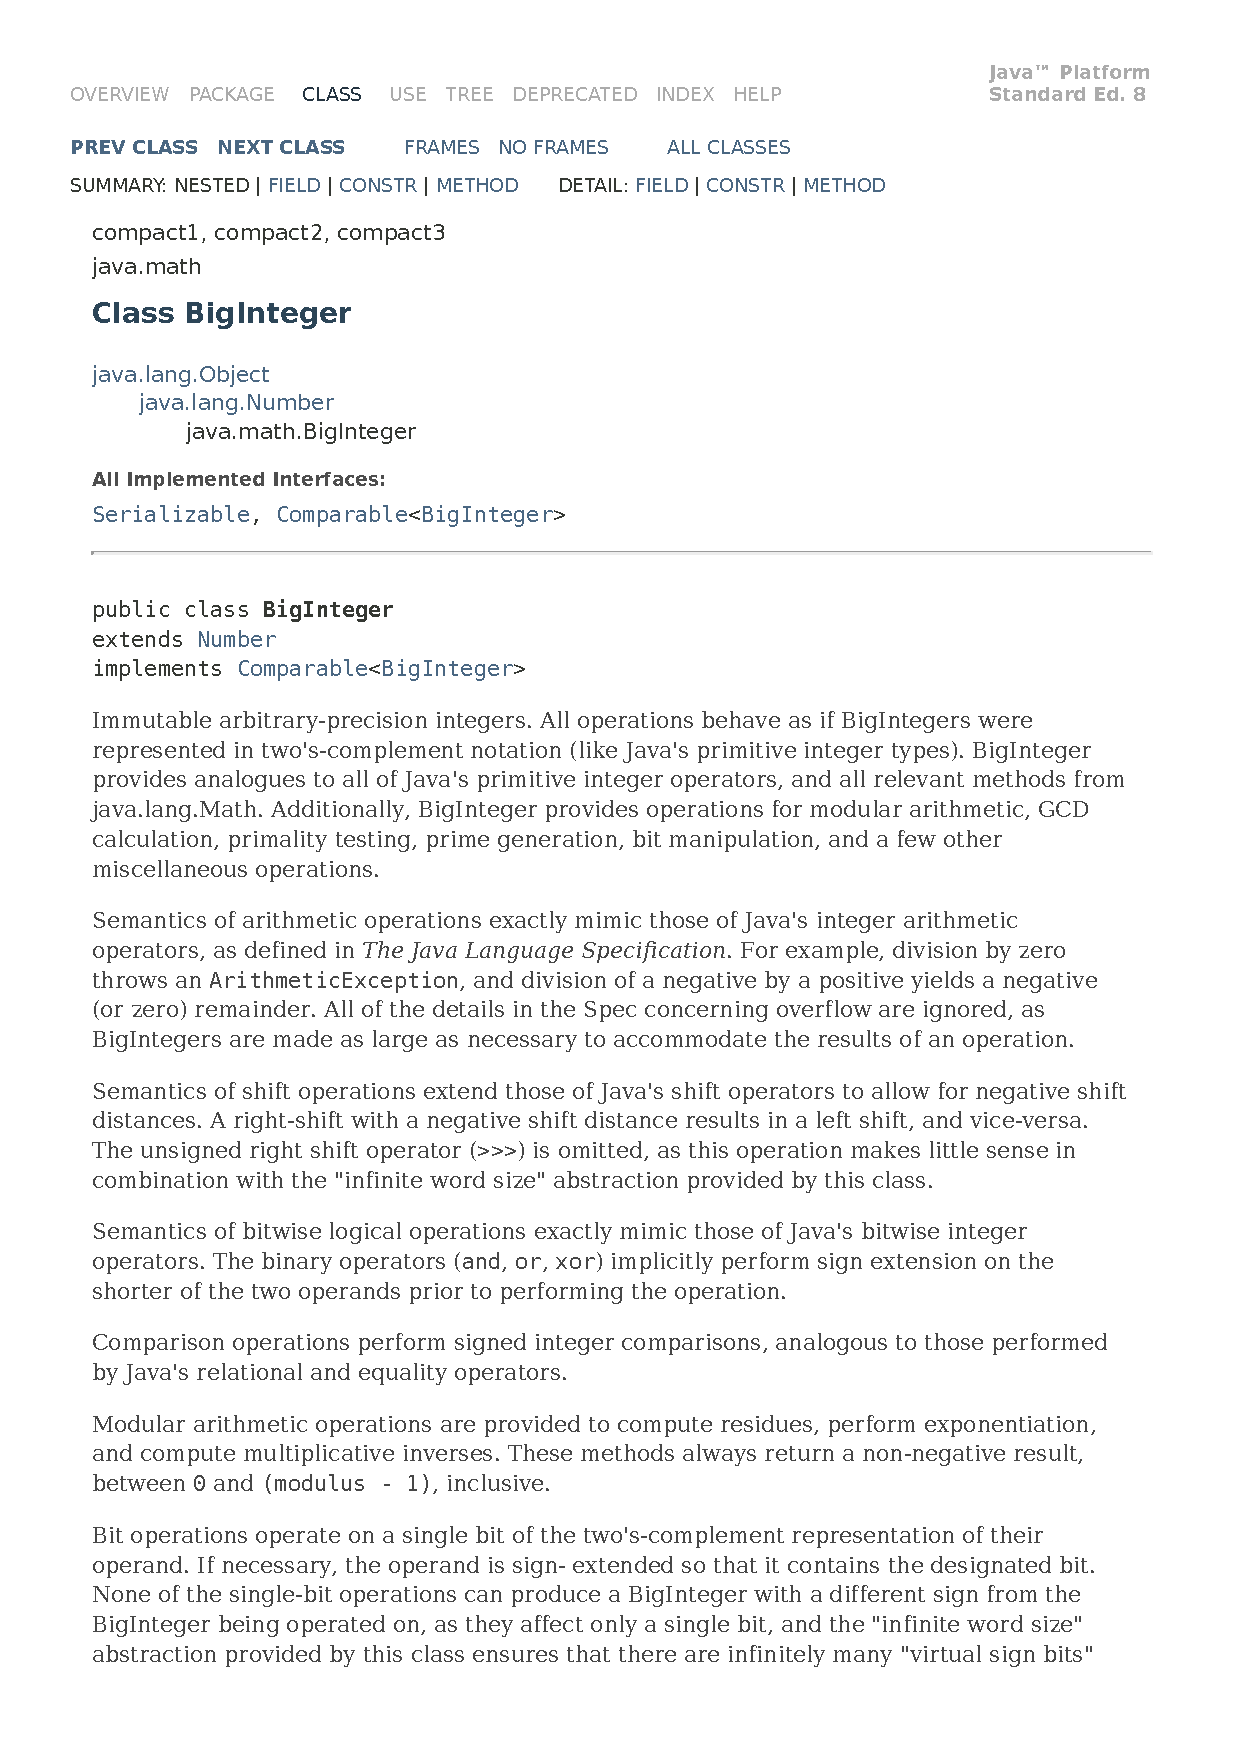
\includepdf[pages={1-6}]{source/biginteger.pdf}
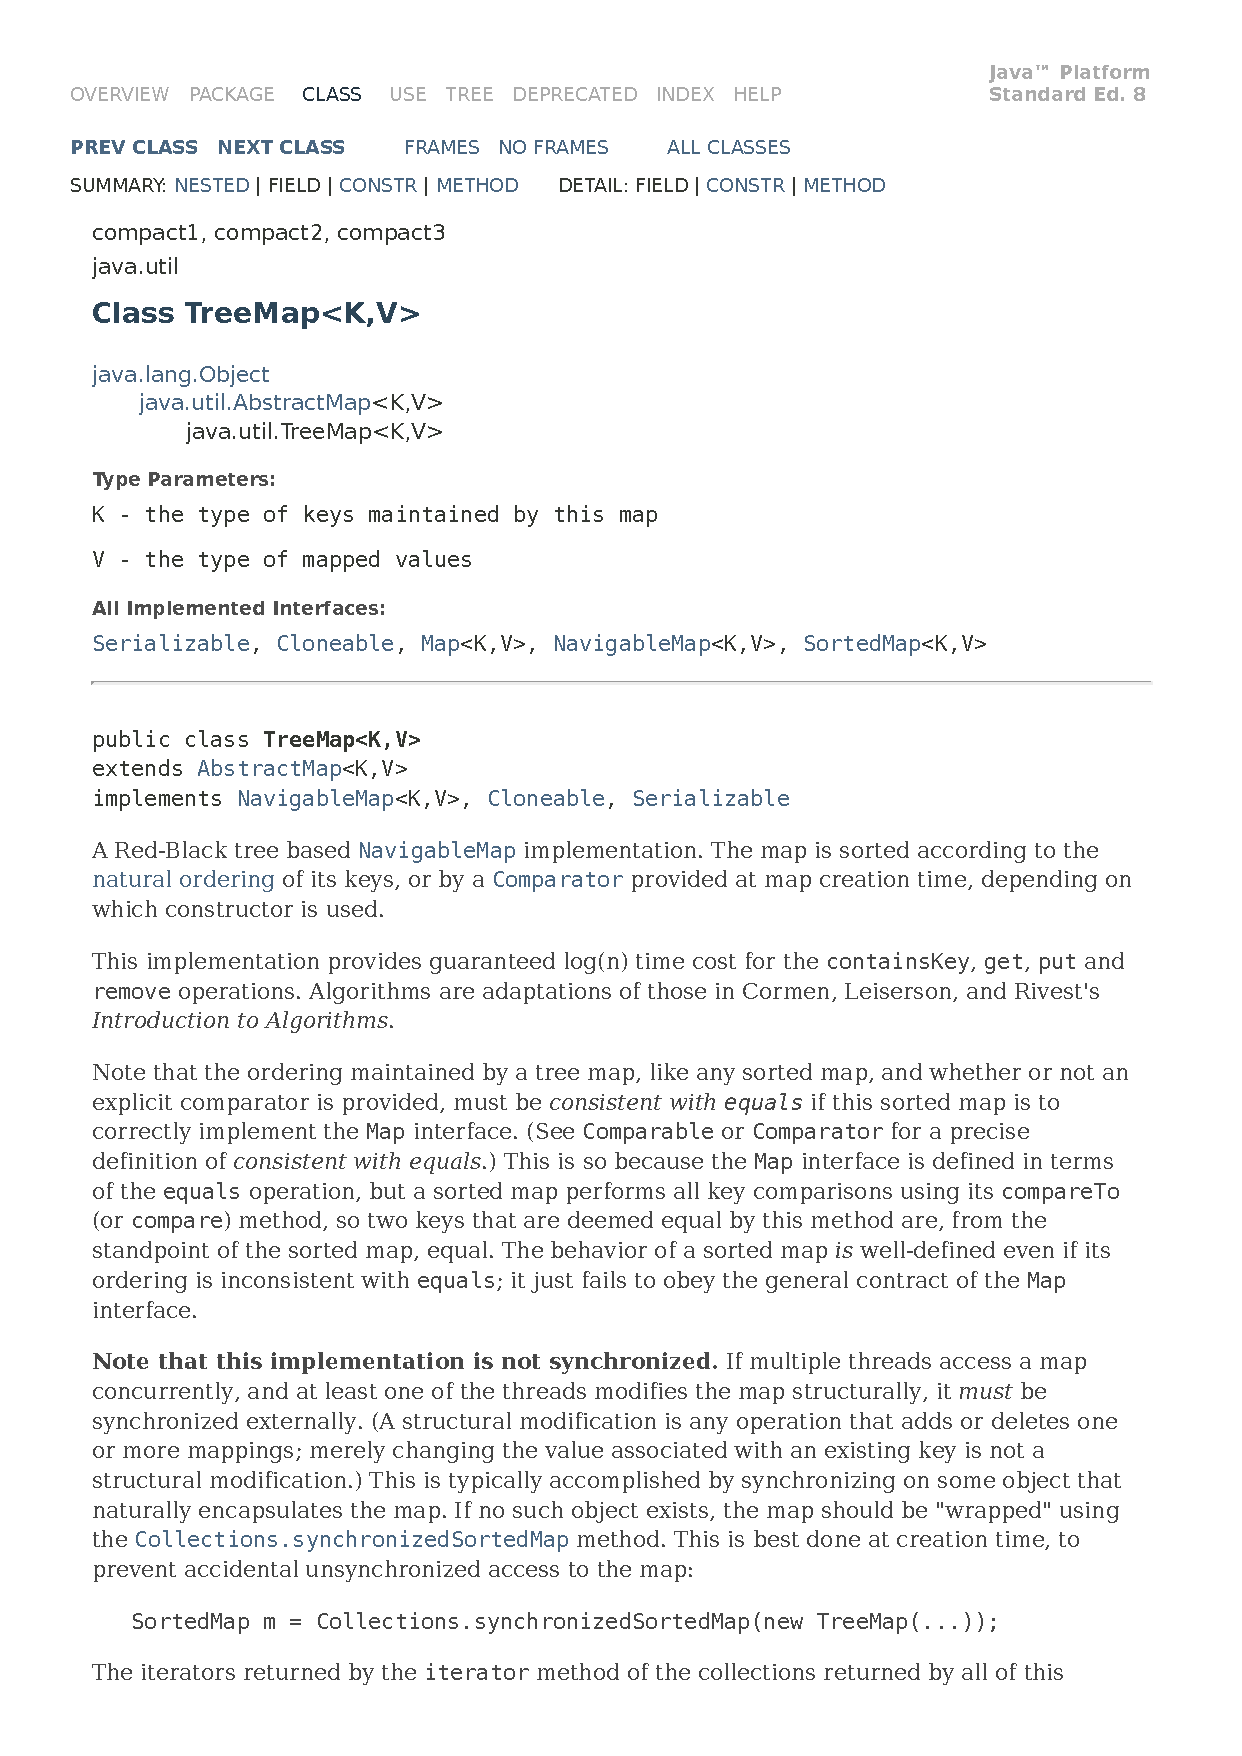
\includepdf[pages={1-5}]{source/treemap.pdf}

\section{gedit}

\javacode{gedit.ini}

%\subsection{BigInteger}

%\subsection{BigDecimal}

\section{数学}

%\subsection{常用积分表}

\subsection{常用数学公式}

\subsubsection{求和公式}

\begin{enumerate}
	\item $\sum_{k=1}^{n}(2k-1)^2 = \frac{n(4n^2-1)}{3}	$
	\item $\sum_{k=1}^{n}k^3 = [\frac{n(n+1)}{2}]^2	$
	\item $\sum_{k=1}^{n}(2k-1)^3 = n^2(2n^2-1)	$
	\item $\sum_{k=1}^{n}k^4 = \frac{n(n+1)(2n+1)(3n^2+3n-1)}{30}  $
	\item $\sum_{k=1}^{n}k^5 = \frac{n^2(n+1)^2(2n^2+2n-1)}{12}	$
	\item $\sum_{k=1}^{n}k(k+1) = \frac{n(n+1)(n+2)}{3}	$
	\item $\sum_{k=1}^{n}k(k+1)(k+2) = \frac{n(n+1)(n+2)(n+3)}{4} $
	\item $\sum_{k=1}^{n}k(k+1)(k+2)(k+3) = \frac{n(n+1)(n+2)(n+3)(n+4)}{5} $
\end{enumerate}

\subsubsection{斐波那契数列}

\begin{enumerate}
	\item $fib_0=0, fib_1=1, fib_n=fib_{n-1}+fib_{n-2}$
	\item $fib_{n+2} \cdot fib_n-fib_{n+1}^2=(-1)^{n+1}$
	\item $fib_{-n}=(-1)^{n-1}fib_n$
	\item $fib_{n+k}=fib_k \cdot fib_{n+1}+fib_{k-1} \cdot fib_n$
	\item $gcd(fib_m, fib_n)=fib_{gcd(m, n)}$
	\item $fib_m|fib_n^2\Leftrightarrow nfib_n|m$
\end{enumerate}

\subsubsection{错排公式}

\begin{enumerate}
	\item $D_n = (n-1)(D_{n-2}-D_{n-1})$
	\item $D_n = n! \cdot (1-\frac{1}{1!}+\frac{1}{2!}-\frac{1}{3!}+\ldots+\frac{(-1)^n}{n!})$
\end{enumerate}

\subsubsection{莫比乌斯函数}

$$\mu(n) = \begin{cases}
1 & \text{若}n=1\\
(-1)^k & \text{若}n\text{无平方数因子,且}n = p_1p_2\dots p_k\\
0 & \text{若}n\text{有大于}1\text{的平方数因数}
\end{cases}$$
$$\sum_{d|n}{\mu(d)} = \begin{cases}
1 & \text{若}n=1\\
0 & \text{其他情况}
\end{cases}$$
$$g(n) = \sum_{d|n}{f(d)} \Leftrightarrow f(n) = \sum_{d|n}{\mu(d)g(\frac{n}{d})}$$
$$g(x) = \sum_{n=1}^{[x]}f(\frac{x}{n}) \Leftrightarrow f(x) = \sum_{n=1}^{[x]}{\mu(n)g(\frac{x}{n})}$$

\subsubsection{伯恩赛德引理}
设$G$是一个有限群,作用在集合$X$上。对每个$g$属于$G$,令$X^g$表示$X$中在$g$作用下的不动元素,轨道数(记作$|X/G|$)由如下公式给出:
$$|X/G| = \frac{1}{|G|}\sum_{g \in G}|X^g|.\,$$

\subsubsection{五边形数定理}

设$p(n)$是$n$的拆分数,有$$p(n) = \sum_{k \in \mathbb{Z} \setminus \{0\}} (-1)^{k - 1} p\left(n - \frac{k(3k - 1)}{2}\right)$$

\subsubsection{树的计数}

\begin{enumerate}
	\item 有根树计数:$n+1$个结点的有根树的个数为
	$$a_{n+1} = \frac{\sum_{j=1}^{n}{j \cdot a_j \cdot{S_{n, j}}}}{n}$$
	其中,
	$$S_{n, j} = \sum_{i=1}^{n/j}{a_{n+1-ij}} = S_{n-j, j} + a_{n+1-j}$$
	\item 无根树计数:当$n$为奇数时,$n$个结点的无根树的个数为
	$$a_n-\sum_{i=1}^{n/2}{a_ia_{n-i}}$$
	当$n$为偶数时,$n$个结点的无根树的个数为
	$$a_n-\sum_{i=1}^{n/2}{a_ia_{n-i}}+\frac{1}{2}a_{\frac{n}{2}}(a_{\frac{n}{2}}+1)$$
	\item $n$个结点的完全图的生成树个数为
	$$n^{n-2}$$
	\item 矩阵-树定理:图$G$由$n$个结点构成,设$\bm{A}[G]$为图$G$的邻接矩阵、$\bm{D}[G]$为图$G$的度数矩阵,则图$G$的不同生成树的个数为$\bm{C}[G] = \bm{D}[G] - \bm{A}[G]$的任意一个$n-1$阶主子式的行列式值。
\end{enumerate}

\subsubsection{欧拉公式}

平面图的顶点个数、边数和面的个数有如下关系:
$$V - E + F = C+ 1$$
\indent 其中,$V$是顶点的数目,$E$是边的数目,$F$是面的数目,$C$是组成图形的连通部分的数目。当图是单连通图的时候,公式简化为:
$$V - E + F = 2$$

\subsubsection{皮克定理}

给定顶点坐标均是整点(或正方形格点)的简单多边形,其面积$A$和内部格点数目$i$、边上格点数目$b$的关系:
$$A = i + \frac{b}{2} - 1$$

\subsubsection{牛顿恒等式}

设$$\prod_{i = 1}^n{(x - x_i)} = a_n + a_{n - 1} x + \dots + a_1 x^{n - 1} + a_0 x^n$$
$$p_k = \sum_{i = 1}^n{x_i^k}$$
则$$a_0 p_k + a_1 p_{k - 1} + \cdots + a_{k - 1} p_1 + k a_k = 0$$

特别地,对于$$|\bm{A} - \lambda \bm{E}| = (-1)^n(a_n + a_{n - 1} \lambda + \cdots + a_1 \lambda^{n - 1} + a_0 \lambda^n)$$
有$$p_k = Tr(\bm{A}^k)$$

%\subsection{数论公式}

\subsection{平面几何公式}

\subsubsection{三角形}

\begin{enumerate}
	\item 半周长
	$$p=\frac{a+b+c}{2}$$
	\item 面积
	$$S=\frac{a \cdot H_a}{2}=\frac{ab \cdot sinC}{2}=\sqrt{p(p-a)(p-b)(p-c)}$$
	\item 中线
	$$M_a=\frac{\sqrt{2(b^2+c^2)-a^2}}{2}=\frac{\sqrt{b^2+c^2+2bc \cdot cosA}}{2}$$
	\item 角平分线 
	$$T_a=\frac{\sqrt{bc \cdot [(b+c)^2-a^2]}}{b+c}=\frac{2bc}{b+c}cos\frac{A}{2}$$
	\item 高线
	$$H_a=bsinC=csinB=\sqrt{b^2-(\frac{a^2+b^2-c^2}{2a})^2}$$
	\item 内切圆半径
	\begin{align*}
	r&=\frac{S}{p}=\frac{arcsin\frac{B}{2} \cdot sin\frac{C}{2}}{sin\frac{B+C}{2}}=4R \cdot sin\frac{A}{2}sin\frac{B}{2}sin\frac{C}{2}\\
	&=\sqrt{\frac{(p-a)(p-b)(p-c)}{p}}=p \cdot tan\frac{A}{2}tan\frac{B}{2}tan\frac{C}{2}
	\end{align*}
	\item 外接圆半径
	$$R=\frac{abc}{4S}=\frac{a}{2sinA}=\frac{b}{2sinB}=\frac{c}{2sinC}$$
\end{enumerate}

\subsubsection{四边形}

$D_1, D_2$为对角线,$M$对角线中点连线,$A$为对角线夹角,$p$为半周长
\begin{enumerate}
	\item $a^2+b^2+c^2+d^2=D_1^2+D_2^2+4M^2$
	\item $S=\frac{1}{2}D_1D_2sinA$
	\item 对于圆内接四边形
	$$ac+bd=D_1D_2$$
	\item 对于圆内接四边形
	$$S=\sqrt{(p-a)(p-b)(p-c)(p-d)}$$
\end{enumerate}

\subsubsection{正$n$边形}

$R$为外接圆半径,$r$为内切圆半径
\begin{enumerate}
	\item 中心角
	$$A=\frac{2\pi}{n}$$
	\item 内角
	$$C=\frac{n-2}{n}\pi$$
	\item 边长
	$$a=2\sqrt{R^2-r^2}=2R \cdot sin\frac{A}{2}=2r \cdot tan\frac{A}{2}$$
	\item 面积
	$$S=\frac{nar}{2}=nr^2 \cdot tan\frac{A}{2}=\frac{nR^2}{2} \cdot sinA=\frac{na^2}{4 \cdot tan\frac{A}{2}}$$
\end{enumerate}

\subsubsection{圆}

\begin{enumerate}
	\item 弧长
	$$l=rA$$
	\item 弦长
	$$a=2\sqrt{2hr-h^2}=2r\cdot sin\frac{A}{2}$$
	\item 弓形高
	$$h=r-\sqrt{r^2-\frac{a^2}{4}}=r(1-cos\frac{A}{2})=\frac{1}{2} \cdot arctan\frac{A}{4}$$
	\item 扇形面积
	$$S_1=\frac{rl}{2}=\frac{r^2A}{2}$$
	\item 弓形面积
	$$S_2=\frac{rl-a(r-h)}{2}=\frac{r^2}{2}(A-sinA)$$
\end{enumerate}

\subsubsection{棱柱}

\begin{enumerate}
	\item 体积
	$$V=Ah$$
	$A$为底面积,$h$为高
	\item 侧面积
	$$S=lp$$
	$l$为棱长,$p$为直截面周长
	\item 全面积
	$$T=S+2A$$
\end{enumerate}

\subsubsection{棱锥}

\begin{enumerate}
	\item 体积
	$$V=Ah$$
	$A$为底面积,$h$为高
	\item 正棱锥侧面积
	$$S=lp$$
	$l$为棱长,$p$为直截面周长
	\item 正棱锥全面积
	$$T=S+2A$$
\end{enumerate}

\subsubsection{棱台}

\begin{enumerate}
	\item 体积
	$$V=(A_1+A_2+\sqrt{A_1A_2}) \cdot \frac{h}{3}$$
	$A_1,A_2$为上下底面积,$h$为高
	\item 正棱台侧面积
	$$S=\frac{p_1+p_2}{2}l$$
	$p_1,p_2$为上下底面周长,$l$为斜高
	\item 正棱台全面积
	$$T=S+A_1+A_2$$
\end{enumerate}

\subsubsection{圆柱}

\begin{enumerate}
	\item 侧面积
	$$S=2\pi rh$$
	\item 全面积
	$$T=2\pi r(h+r)$$
	\item 体积
	$$V=\pi r^2h$$
\end{enumerate}

\subsubsection{圆锥}

\begin{enumerate}
	\item 母线
	$$l=\sqrt{h^2+r^2}$$
	\item 侧面积
	$$S=\pi rl$$
	\item 全面积
	$$T=\pi r(l+r)$$
	\item 体积
	$$V=\frac{\pi}{3} r^2h$$
\end{enumerate}

\subsubsection{圆台}

\begin{enumerate}
	\item 母线
	$$l=\sqrt{h^2+(r_1-r_2)^2}$$
	\item 侧面积
	$$S=\pi(r_1+r_2)l$$
	\item 全面积
	$$T=\pi r_1(l+r_1)+\pi r_2(l+r_2)$$
	\item 体积
	$$V=\frac{\pi}{3}(r_1^2+r_2^2+r_1r_2)h$$
\end{enumerate}

\subsubsection{球}

\begin{enumerate}
	\item 全面积
	$$T=4\pi r^2$$
	\item 体积
	$$V=\frac{4}{3}\pi r^3$$
\end{enumerate}

\subsubsection{球台}

\begin{enumerate}
	\item 侧面积
	$$S=2\pi rh$$
	\item 全面积
	$$T=\pi(2rh+r_1^2+r_2^2)$$
	\item 体积
	$$V=\frac{\pi h[3(r_1^2+r_2^2)+h^2]}{6}$$
\end{enumerate}

\subsubsection{球扇形}

\begin{enumerate}
	\item 全面积
	$$T=\pi r(2h+r_0)$$
	$h$为球冠高,$r_0$为球冠底面半径
	\item 体积
	$$V=\frac{2}{3}\pi r^2h$$
\end{enumerate}

\subsection{立体几何公式}

\subsubsection{球面三角公式}

设$a, b, c$是边长,$A, B, C$是所对的二面角,
有余弦定理$$cos a = cos b \cdot cos c + sin b \cdot sin c \cdot cos A$$
正弦定理$$\frac{sin A}{sin a} = \frac{sin B}{sin b} = \frac{sin C}{sin c}$$
三角形面积是$A + B + C - \pi$

\subsubsection{四面体体积公式}

$U, V, W, u, v, w$是四面体的$6$条棱,$U, V, W$构成三角形,$(U, u), (V, v), (W, w)$互为对棱,
则$$V = \frac{\sqrt{(s - 2a)(s - 2b)(s - 2c)(s - 2d)}}{192 uvw}$$
其中$$\left\{\begin{array}{lll}
a & = & \sqrt{xYZ}, \\
b & = & \sqrt{yZX}, \\
c & = & \sqrt{zXY}, \\
d & = & \sqrt{xyz}, \\
s & = & a + b + c + d, \\ 
X & = & (w - U + v)(U + v + w), \\
x & = & (U - v + w)(v - w + U), \\
Y & = & (u - V + w)(V + w + u), \\
y & = & (V - w + u)(w - u + V), \\
Z & = & (v - W + u)(W + u + v), \\
z & = & (W - u + v)(u - v + W)
\end{array}\right.$$

%\subsection{常用数表}

%\subsubsection{梅森数}

\end{document}
